\documentclass{article}

% Packages for setting up page margins
\usepackage[margin=1in]{geometry}

\usepackage{graphicx, setspace, amsmath, mathtools, amssymb, url, float, listings}
\setlength{\parskip}{2mm}
\graphicspath{ {./images/} }

% Title
\title{CS535 Design and Analysis of Algorithms - Assignment 6}
\author{Batkhishig Dulamsurankhor - A20543498}
\date{\today} % Use \date{} for no date

\begin{document}

\maketitle

\begin{enumerate}
    %q1
    \item To reduce it to bipartite matching problem, we need two sets of vertices such that there is no edge within the sets.
    We can form such a graph by creating two disjoint sets $S_1$ and $S_2$ where these two sets are basically two copies of the original set $S$.
    Then for each edge between $A \in S$ and $B \in S$ in the original graph, we can add edges between $S_1$ and $S_2$ for copies of $A_1 \in S_1$ and $B_2 \in S_2$.

    Our goal is to find a subgraph where every edge has exactly one indegree and outdegree edges.
    This means we need to find a perfect match.
    We can use Hopcroft-Karp algorithm to find maximum matching in the graph.
    If the maximum matching is equal to the number of vertices in $S$, we have the perfect matching.
    Otherwise, it is impossible to find a subgraph where every edge has exactly one indegree and outdegree edges.

    \begin{lstlisting}
        function BFS():
            queue <- new queue
            for s1 in S1:
                if pairS1[s1] == null:
                    dist[s1] = 0
                    queue.add(s1)
            dist[null]=inf
            while !queue.empty:
                s1=queue.poll()
                if dist[s1]<dist[null]:
                    for s2 in adj[s1]:
                        if dist[pairS2[s2]]=inf:
                            dist[pairS2[s2]] = dist[s1]+1
                            queue.add(pair_S2[s2])
            return dist[null]!=inf

        function DFS(s2):
            if s2!=null:
                for s2 in S2:
                    if dist[pair[s2]]=dist[s1]+1:
                        if (DFS(s2))=true:
                            pairS2[s2]=s1
                            pairS1[s1]=s2
                            return true
                dist[s1]=inf
                return false
            return true

        // start here, G(V,E)
        S1 <- copy of V
        S2 <- copy of V
        PairS1 <- empty map
        PairS2 <- empty map
        m <- 0

        while BFS() == true:
            for s1 in S1:
                if pairS1[s1] == null:
                    if DFS(s1) == true:
                        m += 1
        newG <- PairS1, PairS2
        if m==size(G.V):
            return newG
        return false

    \end{lstlisting}

    Example:

    \begin{figure}[H]
        \centering
        \begin{minipage}{0.3\textwidth}
            \centering
            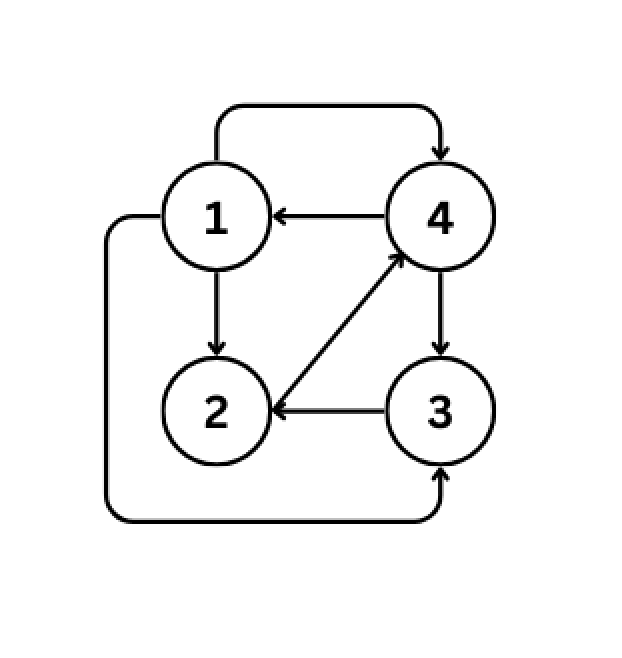
\includegraphics[width=\textwidth]{image1.png}
            \caption{We have above graph. Edges:
                    $(1)\rightarrow(2,3,4)$,
                    $(2)\rightarrow(4)$,
                    $(3)\rightarrow(2)$,
                    $(4)\rightarrow(1,3)$}
        \end{minipage}
        \hspace{0.5cm}
        \begin{minipage}{0.3\textwidth}
            \centering
            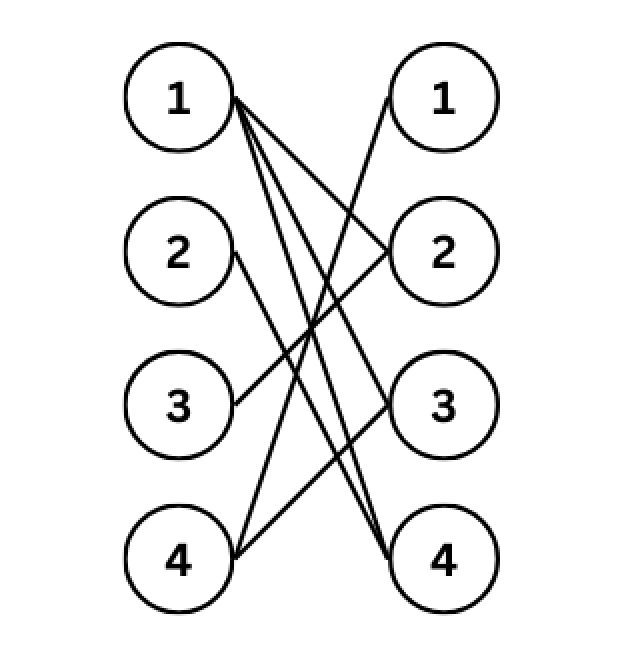
\includegraphics[width=\textwidth]{image2.png}
            \caption{We make two copies of $S$ for $S1$ and $S2$, add edges from $S1$ to $S2$ according to the edges in the graph and create a bipartite graph.}
        \end{minipage}
        \hspace{0.5cm}
        \begin{minipage}{0.3\textwidth}
            \centering
            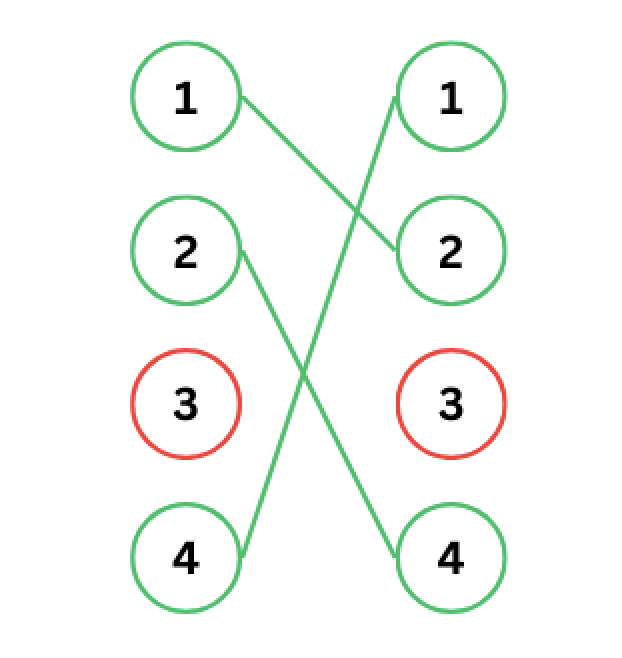
\includegraphics[width=\textwidth]{image3.png}
            \caption{The result after the first iteration. We run BFS for the first time and have total of 3 matched pairs.}
        \end{minipage}
    \end{figure}

    \begin{figure}[H]
        \centering
        \begin{minipage}{0.3\textwidth}
            \centering
            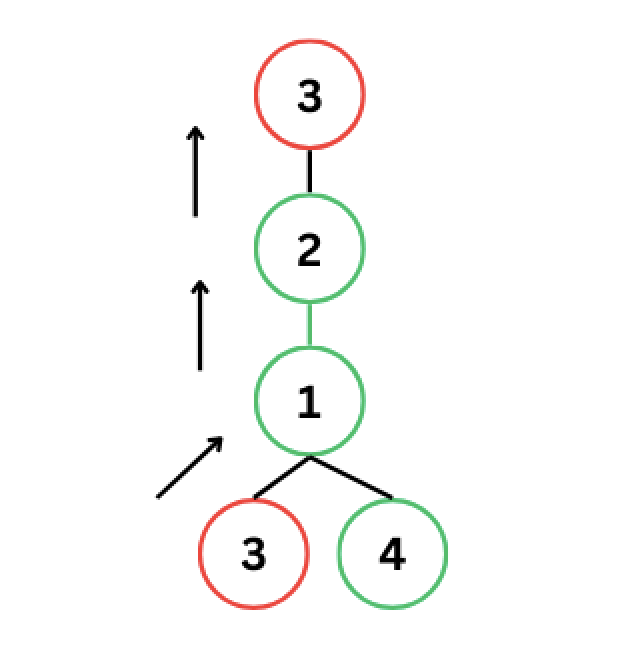
\includegraphics[width=\textwidth]{image4.png}
            \caption{We build augmenting path for the unmatched vertices in $S1$, in this case we have only vertex $(3)$.}
        \end{minipage}
        \hspace{0.5cm}
        \begin{minipage}{0.3\textwidth}
            \centering
            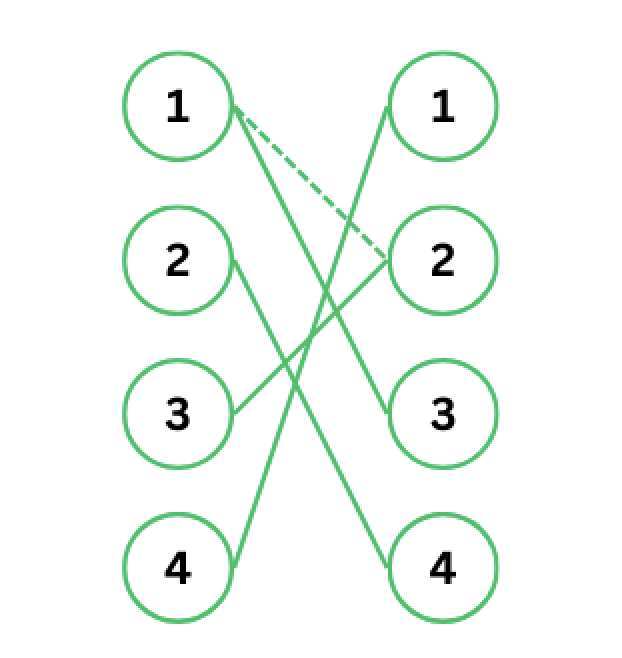
\includegraphics[width=\textwidth]{image5.png}
            \caption{Using the augmenting paths obtained from the previous step, we can run the next iteration and update the mathes.}
        \end{minipage}
        \hspace{0.5cm}
        \begin{minipage}{0.3\textwidth}
            \centering
            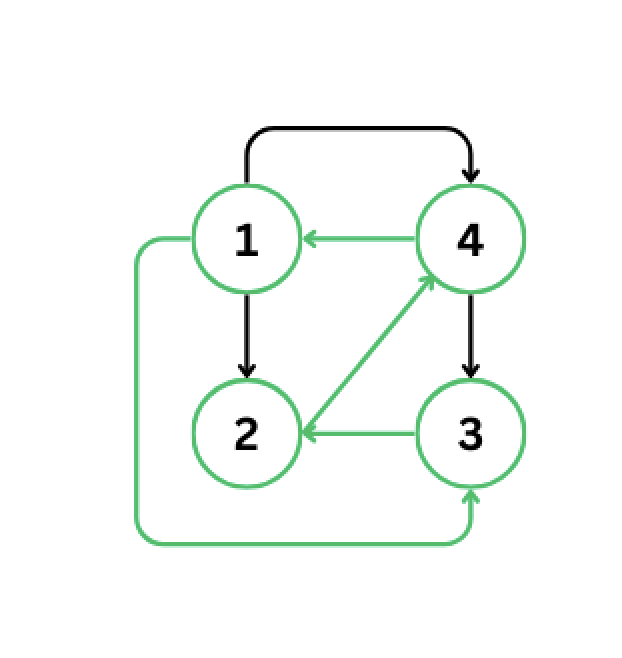
\includegraphics[width=\textwidth]{image6.png}
            \caption{The resulting subset where every edge has exactly one indegree and outdegree edges.}
        \end{minipage}
    \end{figure}

    The time complexity of making a copy of the original subset is $O(V)+O(V)$.
    The time complexity for bfs and dfs is $O(E)$ because in these searches, each edge is considered only once.
    The number iterations the algorithm has to run is $O(\sqrt(V))$ because each iteration increases the length of the shortest augmenting path by at least one \cite{wiki}.
    So, Hopcroft-Karp algorithm runs $O(\sqrt(V)E)$.
    Reconstructing the original graph using the selected pairs takes $O(V)$.
    So, the total time complexity of the algorithm is $O(V)+O(V)+O(\sqrt(V)E)+O(V)=O(\sqrt(V)E)$.

    %q2
    \item 
    
    \begin{enumerate}
        \item Let's say vertex $u$ is in a maximum matching $M^*$ but not in a matching $M$.
        If we find a symmetric difference between them: $M\Delta M^*$, the set contains edges that are only in $M$ or $M^*$ but not in both.
        These alternating edges form paths and cycles.

        We know that $u\in M^*$ so $u$ must be an endpoint in a path, $P$, in the symmetric difference set.
        If the other end of the path $P$ is a matched edge, it must be an alternating path.
        If it's a unmatched vertex, it must be an augmenting path since both $u$ and the other end are unmatched.
        Therefore, if $u$ is unmatched but in $M^*$, it must be either in alternating or augmenting path.
        This is essentially how matching algorithms work by iteratively find augmenting paths and maximize matching.

        \item The algorithm uses bfs and starts from all unmatched vertices from the left side of the bipartite graph.
        It tries to find unmatched edges by finding augmenting path (both ends are unmatched) using dfs.
        If it finds such a path, it augments the path to the current match by flipping the edges in the path.
        Then we have a new path.
        The algorithm keeps on going until there is no such a path left.

        \begin{lstlisting}
            function BFS():
                queue <- new queue
                for s1 in S1:
                    if pairS1[s1] == null:
                        dist[s1] = 0
                        queue.add(s1)
                dist[null]=inf
                while !queue.empty:
                    s1=queue.poll()
                    if dist[s1]<dist[null]:
                        for s2 in adj[s1]:
                            if dist[pairS2[s2]]=inf:
                                dist[pairS2[s2]] = dist[s1]+1
                                queue.add(pair_S2[s2])
                return dist[null]!=inf
    
            function DFS(s2):
                if s2!=null:
                    for s2 in S2:
                        if dist[pair[s2]]=dist[s1]+1:
                            if (DFS(s2))=true:
                                pairS2[s2]=s1
                                pairS1[s1]=s2
                                return true
                    dist[s1]=inf
                    return false
                return true
    
            // start here, G(V,E)
            S1 <- copy of V
            S2 <- copy of V
            PairS1 <- empty map
            PairS2 <- empty map
            m <- 0
    
            while BFS() == true:
                for s1 in S1:
                    if pairS1[s1] == null:
                        if DFS(s1) == true:
                            m += 1
            return m
    
        \end{lstlisting}
    \end{enumerate}

    The time complexity for bfs and dfs is $O(E)$ because in these searches, each edge is considered only once.
    The number iterations the algorithm has to run is $O(\sqrt(V))$ because each iteration increases the length of the shortest augmenting path by at least one \cite{wiki}.
    In thhe worst case, the total time complexity is $O(\sqrt(V)E)$.

    %q3
    \item 
\end{enumerate}

\begin{thebibliography}{9}
    
    \bibitem{wiki}
    Hopcroft-Karp algorithm, \emph{Wikipedia}, \url{https://en.wikipedia.org/wiki/Hopcroft%E2%80%93Karp_algorithm#Analysis}
    
    \end{thebibliography}
\end{document}